\documentclass{article}
\usepackage[utf8]{inputenc}
\usepackage[T1]{fontenc}
\pagestyle{empty}

\title{GenDoc.jl}
\usepackage{tikz}

\begin{document}

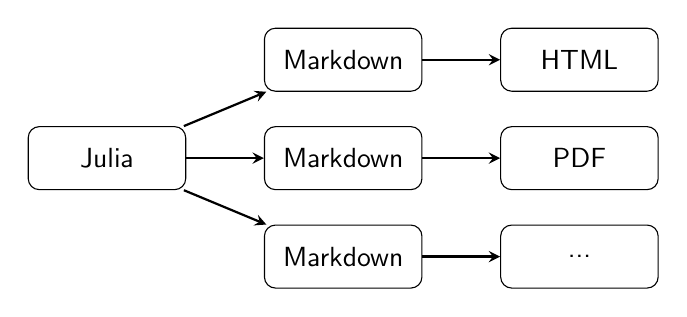
\begin{tikzpicture}[align=center]
\tikzstyle{box} = [rectangle, rounded corners, minimum width=2cm, minimum height=0.8cm, text centered, draw=black]
\tikzstyle{arrow} = [thick,->,>=stealth]
{\fontfamily{cmss}\selectfont
    \path
        (0, 1.25) node[box] (julia) {Julia}
        (3, 2.5) node[box] (markdown) {Markdown}
        (3, 1.25) node[box] (markdown2) {Markdown}
        (3, 0) node[box] (markdown3) {Markdown}
        (6, 2.5) node[box] (html) {HTML}
        (6, 0) node[box] (other) {...}
        (6, 1.25) node[box] (pdf) {PDF};

        \draw [arrow] (julia) -- (markdown);
        \draw [arrow] (julia) -- (markdown2);
        \draw [arrow] (julia) -- (markdown3);
        \draw [arrow] (markdown) -- (html);
        \draw [arrow] (markdown2) -- (pdf);
        \draw [arrow] (markdown3) -- (other);
}
\end{tikzpicture}

\end{document}
